\section{Definite integrals and Fundamental Theorem of Calculus}

In certain application scenarios, we would want to evaluate the area under the curve of a function (bounded by the $x$-axis).  For example, in economics, suppose we have supply and demand curves shown in the graph below, where $P$ stands for price, $Q$ stands for quantity, $D(Q)$ is the demand function, $S(Q)$ is the supply function, and $P^*$, $Q^*$ are the price and demand under equilibrium.  Then the \textit{consumer surplus} is defined as the shaded area marked with "CS", and the \textit{producer surplus} is defined as the shaded area marked with "PS".  It is then clear that the consumer surplus can be evaluated by subtracting $P^*Q^*$ from the area under $D(Q)$ from $Q = 0$ to $Q = Q^*$.  The producer surplus can be calculated as $P^*Q^*$ minus the area under $S(Q)$ from $Q = 0$ to $Q = Q^*$.  Therefore, it would be convenient if we could 
come up with a notation to express areas under curves and develop a technique to evaluate them.

\medskip
\begin{figure}[ht]
    \centering
    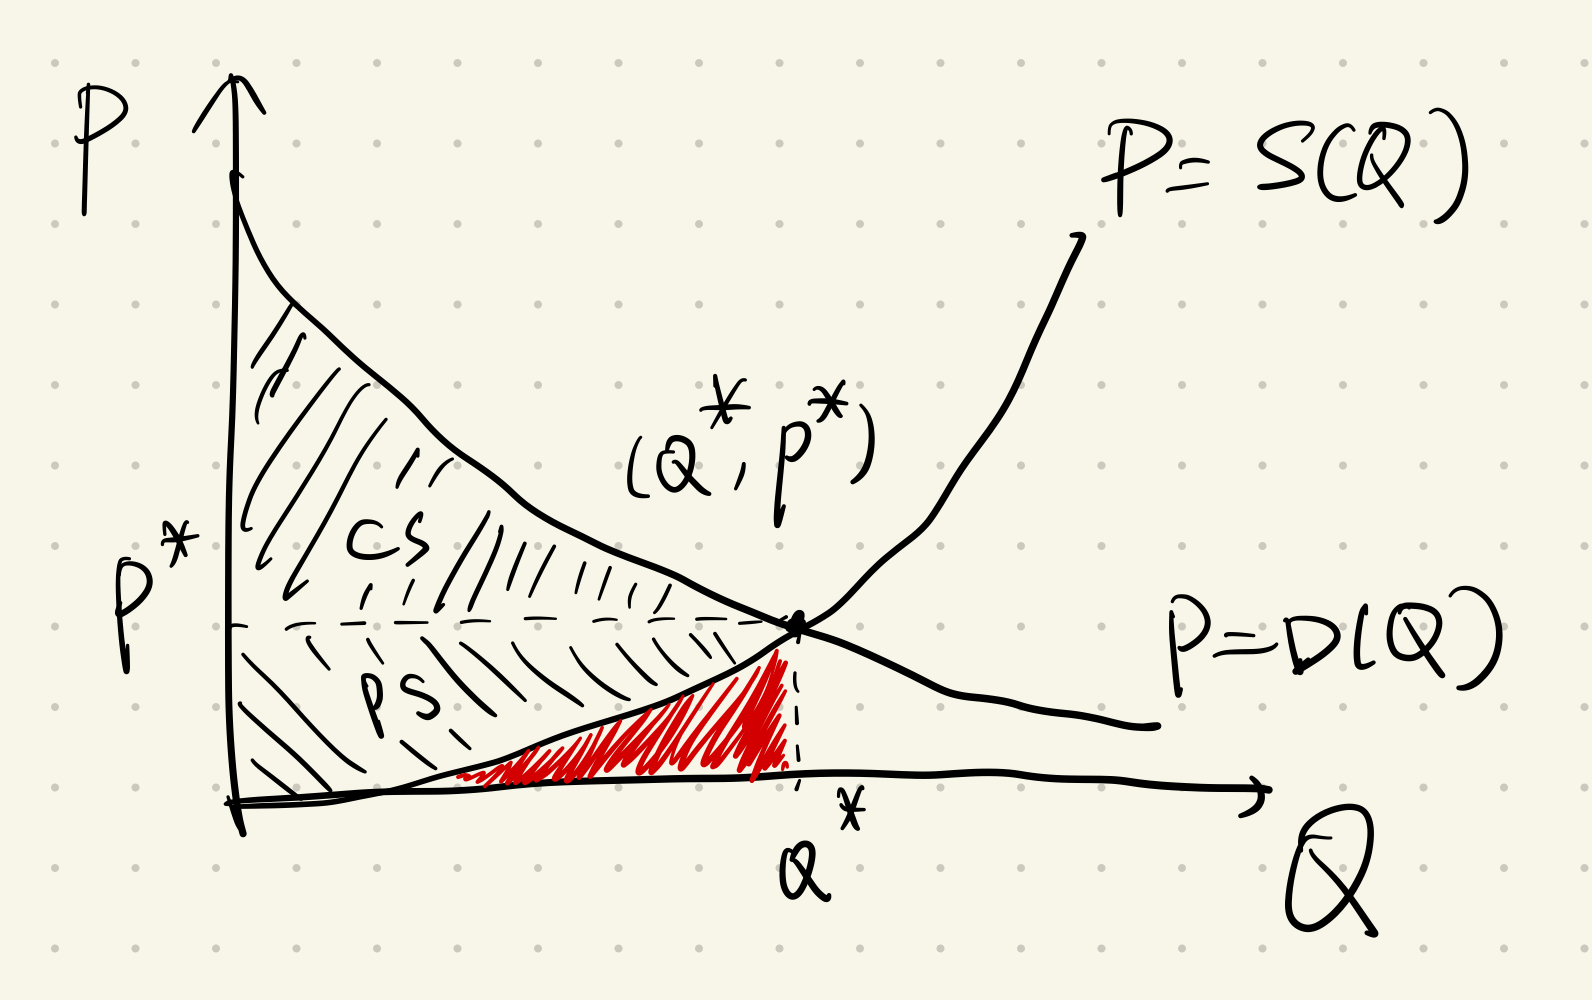
\includegraphics[width = 0.7\textwidth]{figures/chap 07/supply_demand.png}
\end{figure}

\medskip
A side note is that, in the example above, $D(Q)$ and $S(Q)$ are always positive, so it makes sense to talk about area \textit{under} the curve.  However, for functions taking negative values like the what the following graph depicts, the area bound by the curve and the $x$-axis is actually \textit{above} the curve.  In this case, for mathematical consistency, we use the notion of \textbf{signed area}, where areas above the curve and under the $x$-axis like this is given a negative sign.  With the concept of area-under-curve and signed area established, we can now define definite integrals as follows:

\begin{figure}[ht]
    \centering
    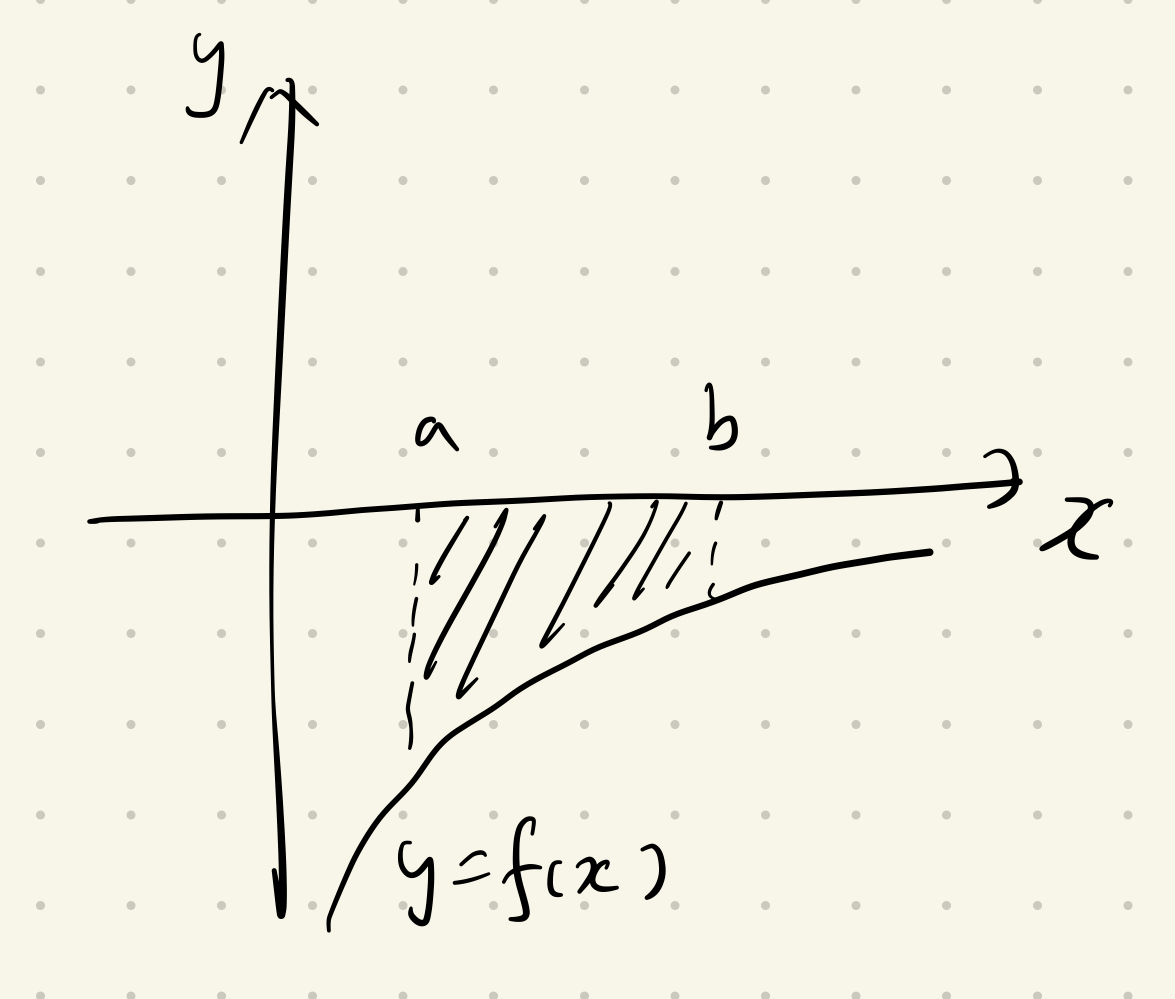
\includegraphics[width = 0.5\textwidth]{figures/chap 07/signed_area.png}
\end{figure}

\begin{defi}[Definite integrals]{def: definite_integral}
    Let $f(x)$ be a continuous function on a closed interval $[a,b]$.  The signed area bounded by the curve of $f(x)$, the $x$-axis, $x=a$ and $x=b$ is called the \textbf{definite integral} of $f(x)$ from $a$ to $b$, denoted by
    \[\int_a^b f(x)~dx\]
    where $a$ and $b$ are termed the lower and upper limit of integration for the definite integral.
\end{defi}

From this definition, if we go back to our previous example, we can notate the cosumer and producer surplus by:
\begin{align*}
    \text{Consumer surplus} &= \Big[\int_0^{Q^*} D(Q) dQ\Big] - P^*Q^*\\
    \text{Producer surplus} &= P^*Q^* - \Big[\int_0^{Q^*} S(Q) dQ\Big]
\end{align*}

Note that since definite integrals represent areas under curve, we have the following identities for definite integrals:
\begin{itemize}
    \item $\int_a^b kf(x)~dx = k\int_a^b f(x)~dx$
    \item $\int_a^b [f(x) \pm g(x)]~dx = \int_a^b f(x)~dx \pm \int_a^b g(x)~dx$
    \item $\int_a^b f(x)~dx = \int_a^c f(x)~dx + \int_c^b f(x)~dx$
    \item $\int_a^a f(x)~dx = 0$
    \item $\int_a^b f(x)~dx = -\int_b^a f(x)~dx$
\end{itemize}
where in the third identity, the area under $f(x)$ between $x = a$ and $x = b$ is intuitively decomposed into the sum of area under curve between $x = a$ and $x = c$, and area under curve between $x = c$ and $x = b$.  Setting $c = a$ in the third identity would lead to 
\[\int_a^b f(x)~dx = \int_a^a f(x)~dx + \int_a^b f(x)~dx\]
\[0 = \int_a^a f(x)~dx\]
which is exactly the fourth identity.  Setting $b = a$ in the third identity would instead lead to
\[\int_a^a f(x)~dx = \int_a^c f(x)~dx + \int_c^a f(x)~dx\]
\[\int_c^a f(x)~dx = -\int_a^c f(x)~dx \]
which implies the fifth identity: switching the upper and lower limit of a definite integral adds a negative sign to it. 

Some definite integrals can be evaluated using our knowledge in geometry.  Let's look at the following examples:

\begin{eg}[]{eg: definite_integrals}
    Using the definition of definite integrals, evaluate the following expressions:
    \begin{tasks}(3)
        \task $\int_0^2 (3x+1)~dx$
        \task $\int_2^4 (2x-5)~dx$
        \task $\int_3^1 \sqrt{4-(x-1)^2}~dx$
    \end{tasks}
\end{eg}

\begin{egsol}[]{egsol: definite_integrals}
    \begin{enumerate}[a)]
        \item If we graph $f(x) = 3x+1$ on the Cartesian plane, we see that the area under the curve from $x=0$ to $x=2$ forms a trapezoid shown in the graph below.  The two bases of the trapezoid are $f(0) = 1$ and $f(2) = 7$, and its height is $2$, so the area would be $\frac{(7+1)\cdot 2}{2} = 8$.  Therefore, the definite integral evaluates to $8$.

        \medskip
        \begin{center}
            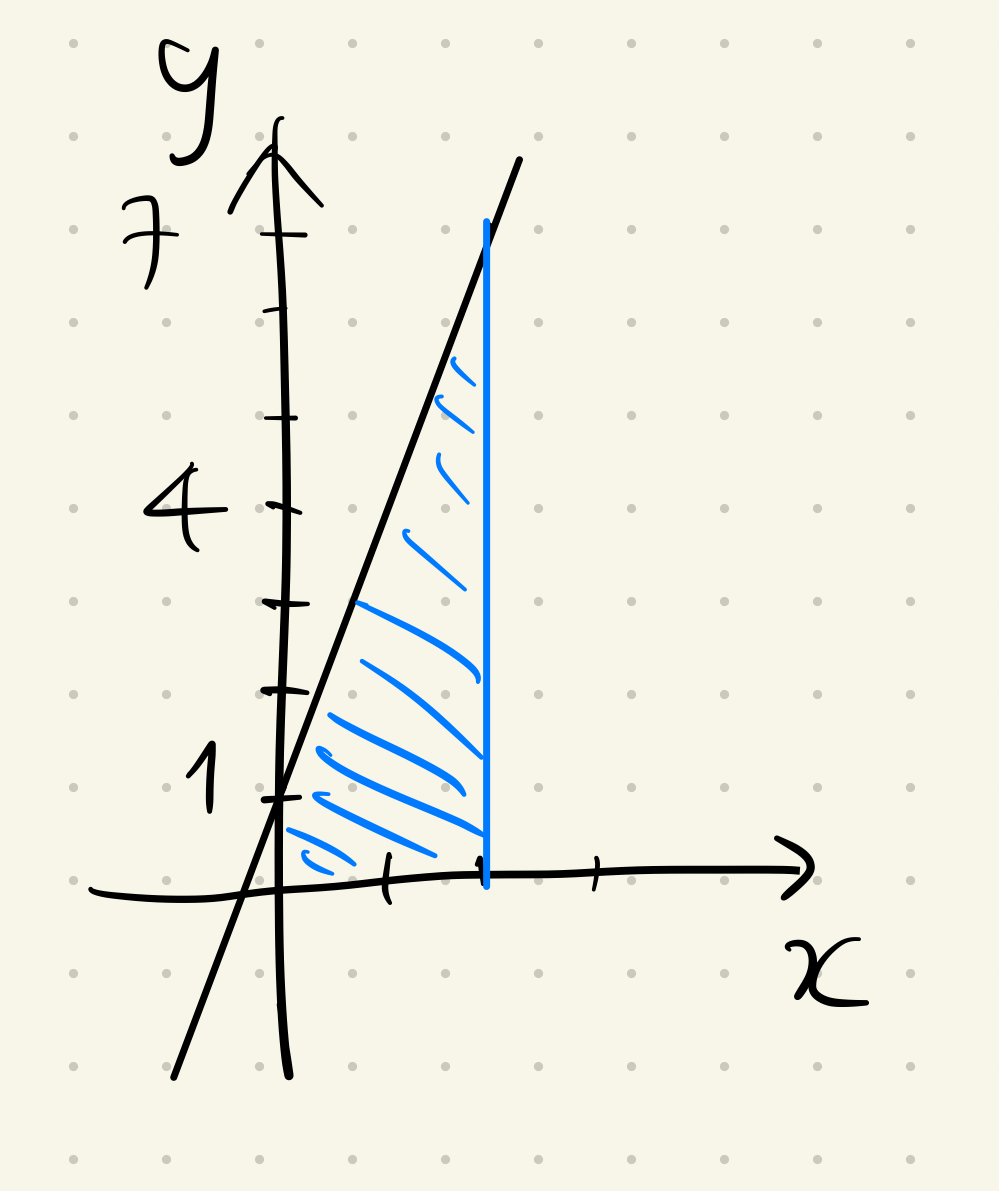
\includegraphics[width = 0.3\textwidth]{figures/chap 07/def_int_a.png}
        \end{center}
        \item If we graph $f(x) = 2x-5$ on the Cartesian plane, we see that between $x = 2$ and $x = 4$, part of the function is below the $x$-axis, and part of it is above the axis.  Since definite integrals are defined as signed area under the curves, we'll have to subtract the triangle below the axis from the triangle above the axis.  Using the identity of similar triangles, we know that since the height of the two triangles are $f(4) = 3$ and $|f(2)|=1$, their bases should be $2\cdot\frac{3}{1+3} = \frac{3}{2}$ and $2\cdot\frac{1}{1+3} = \frac{1}{2}$.  Therefore, the definite integral should evaluate to $\frac{3\cdot3/2}{2}-\frac{1\cdot1/2}{2} = 2$.
        
        \medskip
        \begin{center}
            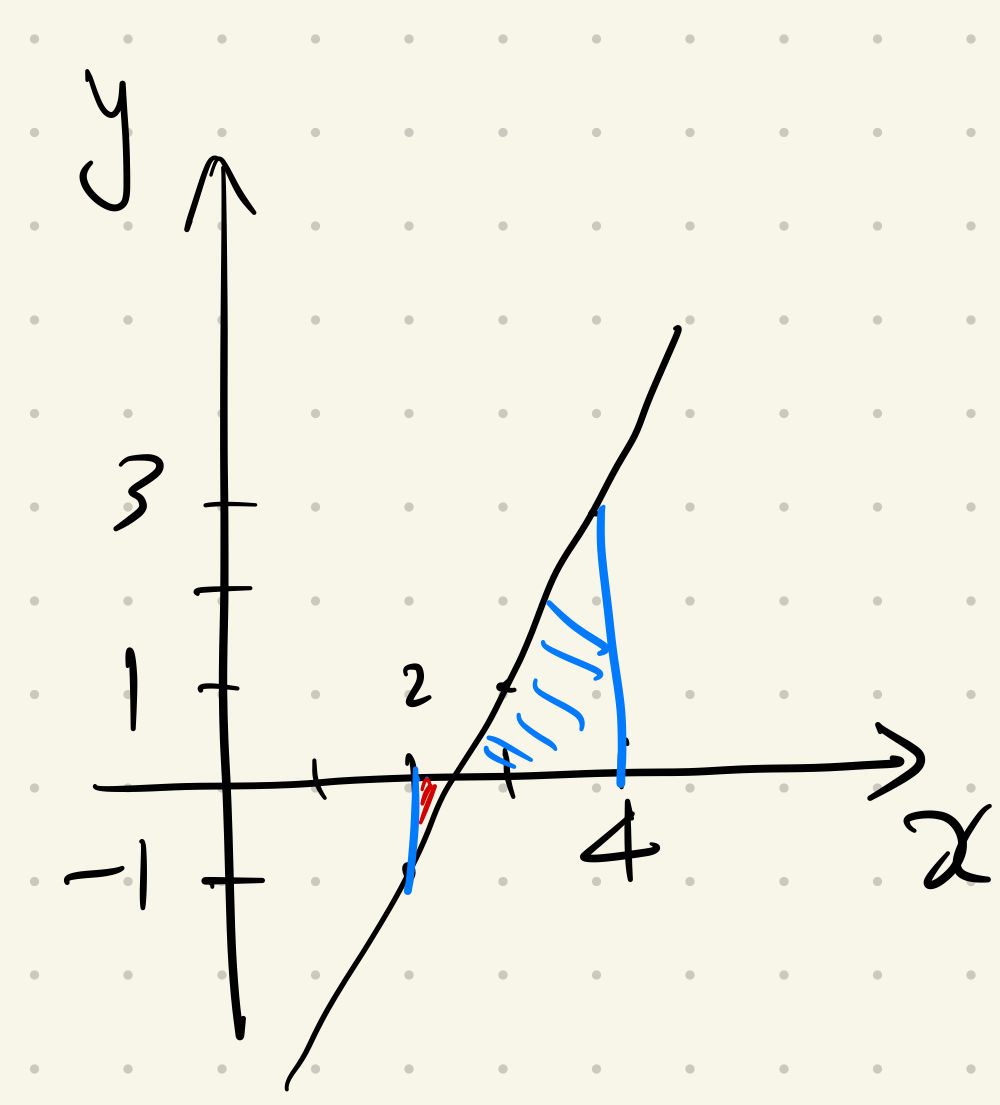
\includegraphics[width = 0.3\textwidth]{figures/chap 07/def_int_b.png}
        \end{center}
        \item Before we start graphing the function, note that upper limit of integration is smaller than its lower limit of integration, which is against our original definition.  However, using the identity we derived above, we can write
        \[\int_3^1 \sqrt{4-(x-1)^2}~dx = - \int_1^3 \sqrt{4-(x-1)^2}~dx\]
        Now the upper limit is larger than the lower limit, we can graph $f(x) = \sqrt{4 - (x-1)^2}$ on the Cartesian plane.  Rearranging $y = \sqrt{4 - (x-1)^2}$ yields $(x-1)^2 + y^2 = 2^2$, which implies that the curve of $f(x)$ is a half circle centered at $(1,0)$ with radius $2$.  Therefore, the area under the curve between $x=1$ and $x=3$ is a quarter of the circle, which has area $\pi\cdot(2)^2/4 = \pi$.  Therefore, our original definite integral evaluates to $-\pi$.
        
        \medskip
        \begin{center}
            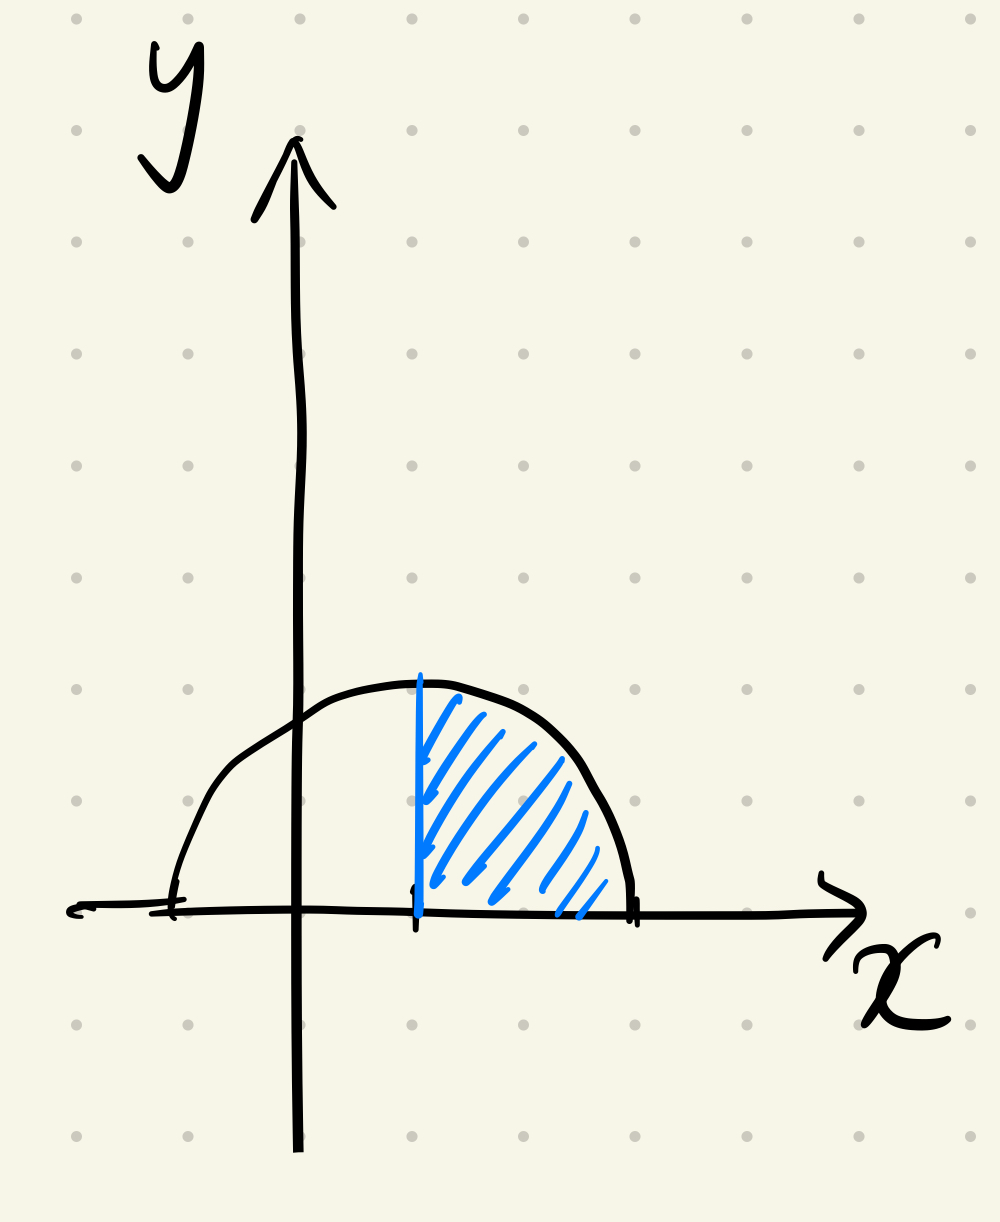
\includegraphics[width = 0.3\textwidth]{figures/chap 07/def_int_c.png}
        \end{center}
    \end{enumerate}
\end{egsol}

In the example above, the functions to be integrated represent straight lines and circles, so the area under the curves all formed shapes we are familiar with.  However, when the functions do not represent lines and circles, evaluating the integral will be much more difficult.  For example, suppose we would like to like to evaluate $\int_0^2 x^2~dx$, whose integrand is a upward-facing parabola as shown in the graph below.  One way to approach the area under curve is to first split the integration interval into smaller subintervals.  For example, in the graph, we split $[0, 2]$ into $8$ subintervals of length $\Delta x_{(8)} = 2/8$.  Then, the area under the curve can be approximated by the sum of the area of the blue bars, each with width $\Delta x_{(8)}$ and height $f(0 + j \Delta x_{(8)})$, where $j$ is the index of the subintervals ranging from $1$ to $8$.  We can write the approximation as
\begin{align*}
    \hat{A}_8 &= (f(0 + \Delta x_{(8)}) + f(0 + 2\Delta x_{(8)}) + f(0 + 3\Delta x) + ... + f(0 + 8 \Delta x_{(8)}))\Delta x_{(8)}\\
    &= \Big[\sum_{j=1}^8 f(0+j \Delta x_{(8)})\Big]\Delta x_{(8)}\\
    &= \Big[\sum_{j=1}^8 j^2 \Delta x_{(8)}^2\Big]\Delta x_{(8)}\\
    &= \Big[\sum_{j=1}^8 j^2\Big] \Delta x_{(8)}^3 =  \Big[\sum_{j=1}^8 j^2\Big] \Big(\frac{2}{8}\Big)^3 = 204 \cdot \Big(\frac{1}{4}\Big)^3 = \frac{51}{16}
\end{align*}

\begin{figure}[ht]
    \centering
    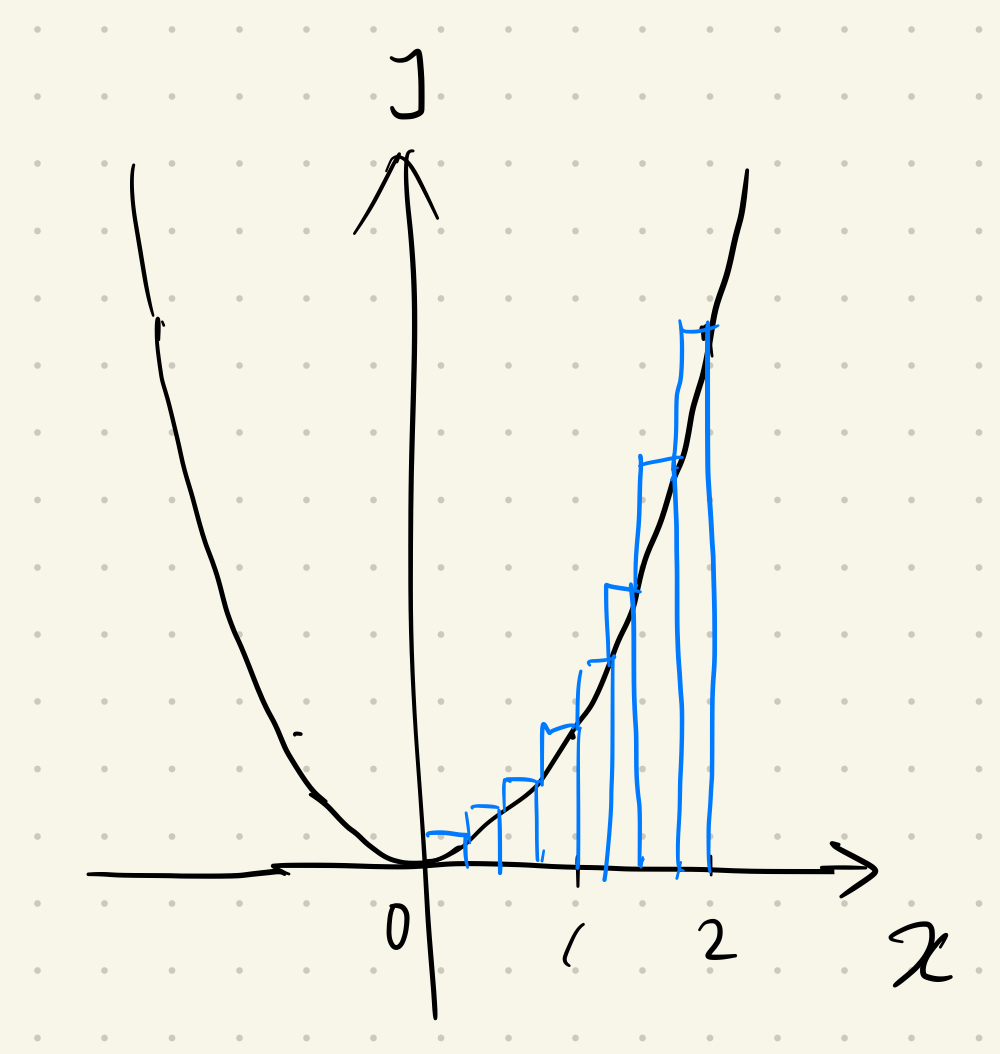
\includegraphics[width = 0.45\textwidth]{figures/chap 07/def_int_series.png}
\end{figure}

This approximation is called a (right) Riemann sum.  If we notate the number of subintervals as $n$ so that the length of the subintervals is $\Delta x_{(n)} = 2/n$, we yield a generalized Riemann sum:
\[\hat{A}_n = \Big[\sum_{j=1}^n j^2\Big] \Delta x_{(n)}^3 = \frac{n(n+1)(2n+1)}{6} \Big(\frac{2}{n}\Big)^3 = \frac{4n(n+1)(2n+1)}{3n^3}\]
where the second equality uses the formula for sum of squares of the first $n$ positive numbers.  Note as $n$ increases, the bars will be finer and finer, and the sum of the bars will eventually approach to the area under the curve.  Therefore, we can write our definite integral as a limit with $n$ approaching infinity:
\[\int_0^2 x^2~dx = \lim_{n \rightarrow \infty} \hat{A}_n = \lim_{n \rightarrow \infty} \frac{4n(n+1)(2n+1)}{3n^3} = \frac{8}{3}\]
where the last equality comes from the ratio of leading coefficients.

Here, we used the limit of Riemann sums to evaluate the definite integral, which is not an easy feat.  However, our success is not without luck: because our integrand is $x^2$, the sum of squares of the first $n$ positive numbers appeared in the Riemann sum, which we happened to know a clean formula for the sum.  If our integrand was something gnarlier, then it may well be the case that we do not have a closed form expression for the Riemann sum, and thus cannot take its limit.  In light of this, we will need a more general procedure to evaluate definite integrals. 

To develop the procedure, first we define an \textbf{area function} as a definite integral that leaves its upper limit as input.  For example, in the graph below, we define the area function $F(x) = \int_0^x f(t)~dt$, where the lower limit of integration is fixed at $0$ but the upper limit of integration is the variable $x$.  The signed area $F(x)$ represents is then by definition the area shaded blue.  

\begin{figure}[ht]
    \centering
    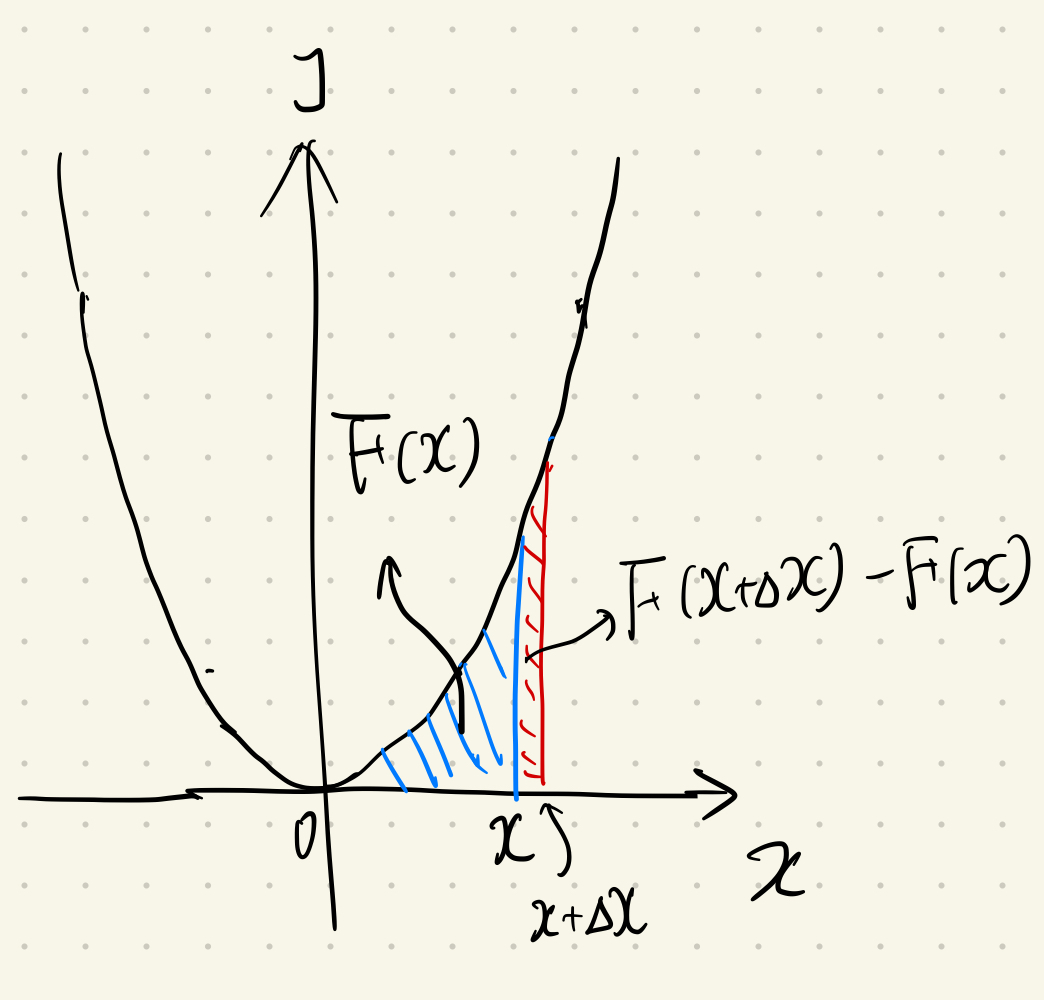
\includegraphics[width = 0.45\textwidth]{figures/chap 07/FTC.png}
\end{figure}

Now for a small $\Delta x$, the difference between $F(x+\Delta x)$ and F(x) would be the small strip of area under curve from $x$ to $x + \Delta x$, which is the area shaded red in the graph.  As $\Delta x$ gets smaller and smaller, the area of the strip would be closer and closer to $f(x) \Delta x$.  In other words, as $\Delta x$ gets smaller and smaller, the ratio between $F(x + \Delta x) - F(x)$ and $\Delta x$ would approach $f(x)$.  Therefore, we have

\[\frac{dF}{dx} = \lim_{\Delta x \rightarrow 0} \frac{F(x + \Delta x) - F(x)}{\Delta x} = f(x)\]

which implies that $F(x)$, which we originally defined as an area function, is actually an antiderivative of $f(x)$!  This remarkable result serves as a bridge between integral calculus (definite integrals) to differential calculus (antiderivatives), which we formally state in the theorem below:

\begin{theo}[Fundamental Theorem of Calculus, First Part]{thm: FTC1}
    Let $f(x)$ be a continuous function on $[a, b]$. Suppose $F(x)$ is an area function defined as 
    \[F(x) = \int_a^x f(t) dt, \quad x \in (a,b)\]
    then $F'(x) = f(x)$ for all $x \in (a,b)$.
\end{theo}

However, note that the first part of the Fundamental Theorem of Calculus only tells us that the area function $F(x)$ is \textit{an} antiderivative of $f(x)$, but does not tell us \textit{which} antiderivative it is.  That is, it does not explicitly tell us what the integration constant should be when we have obtained our antiderivative.  Fortunately, the second part of the Fundamental Theorem of Calculus tells us that as long as we are only interested in evaluating the definite integral, the choice of integration constant does not matter (it also relaxes the requirement for $f(x)$ to be continuous, but here we will not dig deeper into this issue):

\medskip
\begin{theo}[Fundamental Theorem of Calculus, Second Part]{thm: FTC2}
    Let $f(x)$ be a function on $[a, b]$.  Let $F(x)$ be \textit{any} antiderivative for $f(x)$, then
    \[\int_a^b f(x) dx = F(b) - F(a)\]
\end{theo}

Therefore, to find the definite integral for $f(x)$ from $a$ to $b$, we just need to find \textit{one} antiderivative for $f(x)$, and subtract its value at $x = b$ by its value at $x = a$.  Here since antiderivatives are closely linked to the evaluation of definite integrals, they are alternatively termed as \textbf{indefinite integrals}.

Let us try out our new evaluation method for definite integrals with a few examples:

\begin{eg}[]{eg: def_int_FTC}
    Evaluate the following definite integrals
    \begin{tasks}(3)
        \task $\int_0^2 x^2~dx$
        \task $\int_{\pi/2}^{0} \sin x~dx$
        \task $\int_1^{\sqrt{3}} \frac{1}{x^2+1}~dx$
        \task $\int_0^1 \frac{x}{x^2+1}~dx$
        \task $\int_{1/2}^{\sqrt{3}/2} \frac{1}{(\sqrt{1-x^2})^3}~dx$
        \task $\int_{0}^{\pi/4} x \cos x~dx$
    \end{tasks}
\end{eg}

\begin{egsol}[]{egsol: def_int_FTC}
    \begin{enumerate}[a)]
        \item We have evaluated this definite integral the hard way using Riemann sums.  Now let us try using antiderivatives and the Fundamental Theorem of Calculus.  Since one antiderivative of $x^2$ is $\frac{1}{3}x^3$, we can write:
        \[\int_0^2 x^2~dx = \frac{1}{3}x^3\Big]^2_0 = \frac{1}{3}(2)^3 - \frac{1}{3}(0)^3 = \frac{8}{3}\]
        where the notation $g(x)\big]^b_a$ stands for $g(b)-g(a)$.  Antiderivatives have indeed saved us much time here.
        \item Since one antiderivative of $\sin x$ is $-\cos x$, we have
        \[\int_{\pi/2}^0 \sin x~dx = (-\cos x)\Big]_{\pi/2}^0 = -\cos(0) + \cos(\pi/2) = -1 + 0 = -1\]
        Note here we do not even care if the upper limit of integration is larger than the lower limit.  We can just evaluate our antiderivatives with the correct order of subtraction, and the Fundamental Theorem of Calculus will take care of the rest.
        \item Remember that one antiderivative of $\frac{1}{x^2+1}$ is $\arctan x$, so we have
        \[\int_1^{\sqrt{3}} \frac{1}{x^2+1}~dx = \arctan x\Big]_1^{\sqrt{3}} = \arctan(\sqrt{3}) - \arctan(1) = \frac{\pi}{3} - \frac{\pi}{4} = \frac{\pi}{12}\]
        \item The antiderivative for this integrand is not immediately obvious, but if we try U-substituion with $u = x^2+1$, we have $du = 2xdx$, which works since the remainder of the integrand is $x$.  Therefore, we have
        \[\int_0^1 \frac{x}{x^2+1} dx = \frac{1}{2}\int_0^1 \frac{1}{x^2+1}(2xdx)\]
        Now note that when we preform variable substitutions in definite integrals, we will also have to substitute the limits of integration.  That is, originally we are integrating from $x = 0$ to $x = 1$, but now we are changing our variable for integration to $u$, the limits of integration should then be from $u = 0^2+1 = 1$ to $u = 1^2 + 1 = 2$.  We then yield
        \[\frac{1}{2}\int_0^1 \frac{1}{x^2+1}(2xdx) = \frac{1}{2} \int_1^2 \frac{1}{u} du = \frac{1}{2}(\ln |u|)\Big]_1^2 = \frac{1}{2}(\ln |2| - \ln |1|) = \frac{\ln 2}{2}\]
        \item The $\sqrt{1-x^2}$ in the denominator screams for a trigonometric substitution where $x = \sin \theta$ and $dx = \cos \theta d\theta$, but note that since we are performing variable substitution, we need to also transform the limits of integration.  This is where the range setting for $\theta$ becomes important.  Since we by convention set $-\pi/2 \le \theta \le \pi/2$, we have when $x = 1/2$ and $\sqrt{3}/2$, $\theta = \pi/6$ and $\pi/3$. Therefore we yield
        \begin{align*}
            \int_{1/2}^{\sqrt{3}/2} \frac{1}{(\sqrt{1-x^2})^3}~dx &= \int_{\pi/6}^{\pi/3} \frac{1}{\cos^3 \theta}\cos \theta d\theta\\
            &= \int_{\pi/6}^{\pi/3} \sec^2 \theta d\theta\\
            &= \tan \theta \Big]_{\pi/6}^{\pi/3}\\
            &= \tan\Big(\frac{\pi}{3}\Big) - \tan\Big(\frac{\pi}{3}\Big) = \sqrt{3} - \frac{1}{\sqrt{3}} = \frac{2}{3}\sqrt{3}
        \end{align*}
        \item Here the antiderivative can be found using integration by parts setting $u = x$ and $dv/dx = \cos x$, so that $du/dx = 1$ and $v = \sin x$.  Therefore we have
        \begin{align*}
            \int_{0}^{\pi/4} x \cos x~dx &= x \sin x \Big]_{0}^{\pi/4} - \int_{0}^{\pi/4} \sin x~dx\\
            &= x \sin x \Big]_{0}^{\pi/4} + \int_{0}^{\pi/4} (-\sin x)~dx\\
            &= x \sin x \Big]_{0}^{\pi/4} + \cos x \Big]_{0}^{\pi/4}\\
            &= \Big(\frac{\pi}{4} \sin \frac{\pi}{4} - 0 \sin 0\Big) + \Big(\cos \frac{\pi}{4} - \cos 0 \Big)\\
            &= \frac{\pi}{4} \cdot \frac{\sqrt{2}}{2} + \frac{\sqrt{2}}{2} - 1 = \frac{\sqrt{2}}{8}\pi + \frac{\sqrt{2}}{2}- 1
        \end{align*}
        Note that since this is a definite integral, the "$uv$" term is also subject to calculation of value difference at limits of integration, so don't forget to put a right bracket beside it!
    \end{enumerate}
\end{egsol}